\begin{DoxyDate}{Date}
11.\+03.\+2015r. 
\end{DoxyDate}
\begin{DoxyVersion}{Version}
0.\+1 
\end{DoxyVersion}
\hypertarget{_sprawozdanie_Zadanie}{}\section{Zadanie}\label{_sprawozdanie_Zadanie}
\begin{DoxyVerb} Celem ćwiczenia było stworzenie programu benchmarkującego , który dla wybranych danych będzie zliczał średni czas wykonania dowolnego algorytmu ( w tym przypadku mnożenia elementów tablicy przez 2. Należało również stworzyć program generujący losowe liczby.
\end{DoxyVerb}
 \hypertarget{_sprawozdanie_Wyniki}{}\section{Wyniki}\label{_sprawozdanie_Wyniki}
Dla dziesięciu milionów liczb program zwraca 7 danych wyjściowych ( zgodnie z algorytmem 10$^\wedge$n , gdzie n jest równocześnie ilością zwracanych czasów oraz maxymalną liczbą danych dla jakiej przeprowadzany był test

Na podstawie otrzymanych danych mamy \+:


\begin{DoxyImageNoCaption}
  \mbox{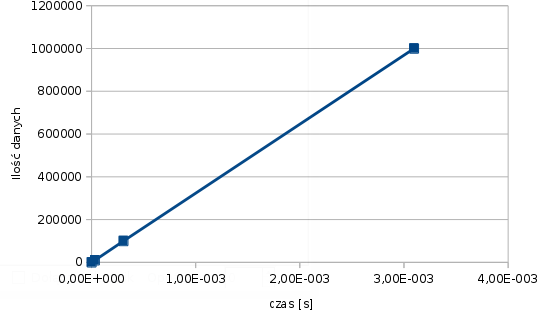
\includegraphics[width=\textwidth,height=\textheight/2,keepaspectratio=true]{1.jpg}}
\end{DoxyImageNoCaption}
\hypertarget{_sprawozdanie_Podsumowanie}{}\section{Podsumowanie}\label{_sprawozdanie_Podsumowanie}
\begin{DoxyVerb} Wykres dodany do dokumentacji z niewiadomych względów nie jest wyświetlany poprawnie ( dodano sprawozdanie również w formacie pdf).
 Zgodnie z przewidywaniami złożoność obliczeniowa jest liniowa , jedyną rzeczą która zwraca uwagę jest fakt iż czas wykonania jednej operacji jest dłuższy od czasu wykonania 10 operacji. Dla wiekszej ilości danych wyniki są poprawne
\end{DoxyVerb}
 Wydaje się , że zbyt mało danych jest obecnych w środkowej częsci wykresu co powinno być zostać zmienione w celu poprawy jakości odbioru wykresu ( dla charakterystyki liniowej jest to akurat bez znaczenia ale .np dla logarytmicznej było by widoczne ). 